\clearpage

\section{시험 입력 생성}\label{sec:engine}

\subsection{기본 개념}

무작위 바이트를 보내는 방식은 대부분 대상의 가장 바깥 형식 검사에서 걸러져, 내부 로직까지 도달하지 못한다.
본 퍼저는 반대로 \textbf{정상 메시지를 출발점으로 삼아 일부만 변형}한다.
메시지의 나머지 부분은 정상이므로 대상의 형식 검사를 통과하고, 변형된 부분이 실제 처리 로직에 도달하게 된다.

하나의 시험(테스트케이스)은 순서가 있는 메시지 단계들로 이루어지며, 각 단계는 ``어떤 메시지의, 어떤 항목을, 어떻게 바꿀 것인가''를 기술한다.
시험 입력은 시드로부터 결정적으로 만들어지므로, 같은 설정으로 다시 실행하면 같은 입력이 재현된다.

\subsection{퍼징 기법}

퍼저는 성격이 다른 다섯 가지 기법을 제공하며, 시험 목적에 따라 조합하여 사용한다.

\begin{table}[H]
\centering
\small
\caption{퍼징 기법}
\label{tab:techniques}
\begin{tabularx}{\textwidth}{l Y}
\toprule
\textbf{기법} & \textbf{개념} \\
\midrule
랜덤 테스트 & 외부에서 관측 가능한 반응만으로 이상 여부를 확인하는 간단한 경계값 시험 \\
생성 메시지 테스트 & 메시지 규격으로부터 경계에 가까운 값이나 선택 항목 변형을 새로 만들어 냄 \\
형식 규칙 테스트 & 메시지 규격을 알고 의도적으로 어김: 타입 혼동, 필수 항목 누락, 허용되지 않은 열거값, 정의되지 않은 항목 추가 \\
정상 샘플 기반 테스트 & 정상 메시지의 항목 값을 바꿔 넣음: 경계값, 다른 식별자, 손상된 값 \\
시퀀스 테스트 & 메시지의 순서 자체를 흔듦: 순서 뒤바꾸기, 선행 단계 생략, 단계 반복, 만료된 식별자 재사용 \\
\bottomrule
\end{tabularx}
\end{table}

변형 대상 항목과 값은 프로토콜 지식에 기반한다.
예를 들어 커넥터 번호와 계량값에는 음수, 시각 항목에는 날짜가 아닌 문자열, 인증 태그에는 등록되지 않은 태그를 넣는 식이다.

웹 화면에서는 시험할 메시지 블록을 누르면 그림~\ref{fig:ui-panel}과 같은 설정 패널이 열린다.
사용자는 여기서 기법을 고르고, 변형의 기준이 될 정상 입력, 변형 비율, 변형 전략 같은 기법별 파라미터를 정한다.
각 파라미터에는 \textbf{추천값 사용} 버튼이 있어 기본 설정으로 바로 시작할 수 있다.

\begin{figure}[H]
    \centering
    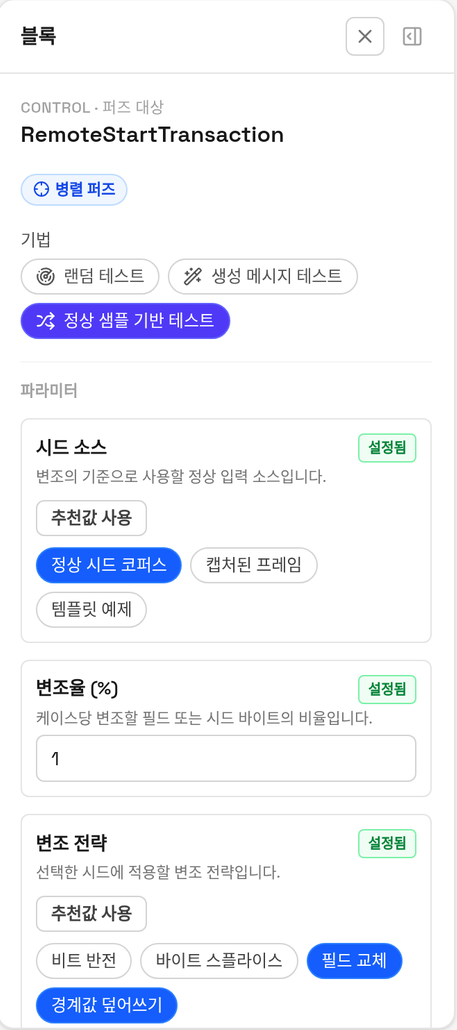
\includegraphics[width=0.42\textwidth]{screenshots/ui02_panel_c.png}
    \caption{웹 화면: 블록별 기법과 파라미터 설정}
    \label{fig:ui-panel}
\end{figure}

\subsection{프로토콜 단계와 시험 범위}

OCPP 충전 세션은 연결·부팅, 인증, 트랜잭션(충전 시작·계량·종료), 원격 제어 단계로 진행되고, ISO 15118은 세션 설정, 서비스 협상, 인증, 충전, 종료 단계로 진행된다.
사용자는 기법마다 \textbf{전체 메시지}, \textbf{특정 단계}, \textbf{특정 메시지} 중 하나로 범위를 정할 수 있다.
이를 통해 ``인증 단계만'' 또는 ``원격 충전 명령만''과 같이 위험도가 높은 부분에 시험을 집중할 수 있다.

\subsection{깊은 상태 시험: 시퀀스와 2단계 캠페인}

많은 결함은 충전이 진행 중이거나 특정 설정이 적용된 \textbf{깊은 상태}에서만 드러난다.
이런 상태에 도달하려면 변형 메시지를 보내기 전에 정상 메시지로 먼저 상태를 만들어야 한다.

퍼저는 이를 \textbf{시퀀스}로 표현한다. 시퀀스는 ``선행 단계 $\rightarrow$ 퍼징 대상 $\rightarrow$ (선택) 리셋''의 체인이며, 매 시험마다 선행 단계는 그대로 재생하고 퍼징 대상에만 새 변형을 적용한다.
리셋은 연결을 끊고 대상이 다시 접속·재부팅하는지를 확인하는 체크포인트이다.

시퀀스의 퍼징 대상에 미리 준비한 공격 메시지가 지정되면 \textbf{2단계 캠페인}으로 동작한다.
앞의 $N-1$회는 대상 메시지를 가볍게 변형하는 준비 시험이고, 마지막 1회만 전체 체인과 함께 공격 메시지를 전달한다.
그림~\ref{fig:sequence}는 충전기에 대한 제조사 정의 데이터 전송 공격을 예로 든 것으로, 선행 단계에서 하트비트 주기를 길게 설정해 공격 도중 세션이 끊기지 않게 한다.

\begin{figure}[H]
\centering
\begin{tikzpicture}[node distance=5mm, every node/.style={font=\footnotesize}]
  \node[box, minimum width=28mm] (b) {설정 조회\\{\scriptsize 선행 단계}};
  \node[box, right=of b, minimum width=34mm] (c) {설정 변경\\{\scriptsize 선행 단계 · 하트비트 주기 연장}};
  \node[hot, right=of c, minimum width=30mm] (f) {데이터 전송 명령\\{\scriptsize 퍼징 대상}};
  \node[ext, right=of f, minimum width=20mm, dashed] (x) {리셋\\{\scriptsize (선택) 재접속}};
  \draw[arr] (b) -- (c); \draw[arr] (c) -- (f); \draw[arr, dashed] (f) -- (x);
  \node[lbl, above=1mm of c] {깊은 상태 형성};
  \node[lbl, above=1mm of f, ksred] {매 시험 새 변형};

  \begin{scope}[yshift=-20mm]
    \foreach \i/\t in {0/1회차,1/2회차,2/$\cdots$,3/$N\!-\!1$회차} {
      \node[box, minimum width=22mm] (p\i) at (\i*26mm,0) {준비 시험\\{\scriptsize \t}};
    }
    \node[hot, minimum width=24mm] (fin) at (4*26mm+2mm,0) {최종 공격\\{\scriptsize $N$회차}};
    \draw[arr] (p0)--(p1); \draw[arr] (p1)--(p2); \draw[arr] (p2)--(p3); \draw[arr] (p3)--(fin);
    \node[lbl, below=1mm of p1, xshift=13mm] {대상 메시지의 항목 하나만 변형};
    \node[lbl, below=1mm of fin] {전체 체인 + 공격 메시지};
  \end{scope}
\end{tikzpicture}
\caption{시퀀스 체인(상)과 2단계 캠페인(하)}
\label{fig:sequence}
\end{figure}

웹 화면에서는 시험을 캔버스 위의 블록 그래프로 구성한다(그림~\ref{fig:ui-graph}).
\textbf{메시지 퍼징} 블록은 메시지 하나를 단독으로 시험하고, \textbf{시퀀스 퍼징}은 퍼징할 메시지를 고르면 그 메시지에 도달하는 데 필요한 선행 단계를 자동으로 만들어 준다.
그림의 아래쪽 줄이 그림~\ref{fig:sequence}의 시퀀스를 그대로 구성한 것이며, 이처럼 미리 준비된 공격 시나리오는 버튼 하나로 불러올 수 있다.
모든 블록의 설정이 끝나면 블록에 ``준비됨''이 표시되고 \textbf{캠페인 실행} 버튼이 활성화된다.

\begin{figure}[H]
    \centering
    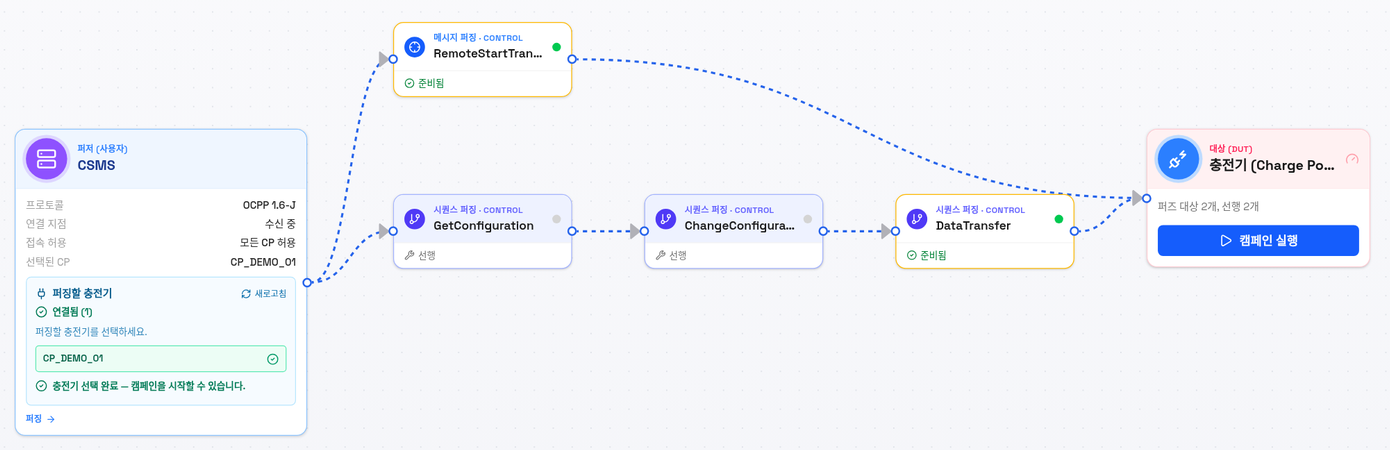
\includegraphics[width=\textwidth]{screenshots/ui02_graph_c.png}
    \caption{웹 화면: 메시지 퍼징 블록(위)과 시퀀스(아래)로 구성한 캠페인}
    \label{fig:ui-graph}
\end{figure}

\subsection{변형 의도 태깅}\label{subsec:tagging}

모든 변형에는 생성 시점에 \textbf{메시지 클래스}라는 의도 태그가 붙는다.
이는 ``이 입력을 받은 대상이 어떻게 반응해야 정상인가''를 미리 적어 둔 것으로, 판정 단계의 기준이 된다.

\begin{itemize}
    \item \textbf{정상 메시지}: 규격 안의 입력. 수락되어야 정상이다.
    \item \textbf{형식은 맞지만 부적합한 메시지}: 형식은 규격에 맞지만 상태·순서·정책상 받아들이면 안 되는 입력. 거부되거나, 최소한 내부 상태를 바꾸지 않아야 정상이다.
    \item \textbf{형식이 깨진 메시지}: 타입 위반, 필수 항목 누락처럼 규격 자체를 어긴 입력. 프로토콜 오류로 거부되어야 정상이다.
\end{itemize}

태그는 변형 방식으로부터 자동으로 정해지며, 판단이 애매하면 ``형식은 맞지만 부적합한 메시지''로 보수적으로 분류한다.
정상 메시지 태그는 시험 작성자가 명시할 때만 붙는다.
